

\tikzset{every picture/.style={line width=0.75pt}} %set default line width to 0.75pt        

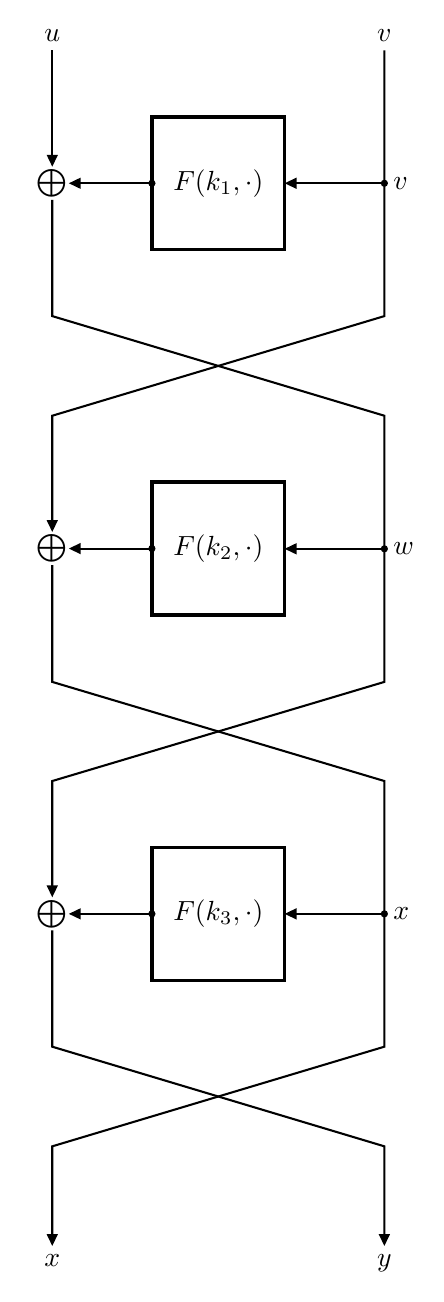
\begin{tikzpicture}[x=0.75pt,y=0.75pt,yscale=-0.8,xscale=0.8]
%uncomment if require: \path (0,871); %set diagram left start at 0, and has height of 871

%Shape: Rectangle [id:dp8324053844032733] 
\draw  [line width=1.2]  (80,80) -- (160,80) -- (160,160) -- (80,160) -- cycle ;
%Straight Lines [id:da3381133919904238] 
\draw    (20,129.96) -- (20,200) -- (220,260) -- (220,420.31) -- (20,480) -- (20,547) ;
\draw [shift={(20,550)}, rotate = 270] [fill={rgb, 255:red, 0; green, 0; blue, 0 }  ][line width=0.08]  [draw opacity=0] (7.14,-3.43) -- (0,0) -- (7.14,3.43) -- cycle    ;
%Shape: Rectangle [id:dp4262407576378149] 
\draw  [line width=1.2]  (80,300) -- (160,300) -- (160,380) -- (80,380) -- cycle ;
%Shape: Rectangle [id:dp3903301490910347] 
\draw  [line width=1.2]  (80,520) -- (160,520) -- (160,600) -- (80,600) -- cycle ;
%Straight Lines [id:da30498630007993843] 
\draw    (220,40) -- (220,200) -- (20,260) -- (20,327) ;
\draw [shift={(20,330)}, rotate = 270] [fill={rgb, 255:red, 0; green, 0; blue, 0 }  ][line width=0.08]  [draw opacity=0] (7.14,-3.43) -- (0,0) -- (7.14,3.43) -- cycle    ;
%Straight Lines [id:da7176994176518701] 
\draw    (20,40) -- (20,107) ;
\draw [shift={(20,110)}, rotate = 270] [fill={rgb, 255:red, 0; green, 0; blue, 0 }  ][line width=0.08]  [draw opacity=0] (7.14,-3.43) -- (0,0) -- (7.14,3.43) -- cycle    ;
%Straight Lines [id:da7838296171746812] 
\draw    (20,570) -- (20,640) -- (220,700) -- (220,757) ;
\draw [shift={(220,760)}, rotate = 270] [fill={rgb, 255:red, 0; green, 0; blue, 0 }  ][line width=0.08]  [draw opacity=0] (7.14,-3.43) -- (0,0) -- (7.14,3.43) -- cycle    ;
%Straight Lines [id:da6843238736783963] 
\draw    (20,350) -- (20,420.31) -- (220,480) -- (220,640) -- (20,700) -- (20,757) ;
\draw [shift={(20,760)}, rotate = 270] [fill={rgb, 255:red, 0; green, 0; blue, 0 }  ][line width=0.08]  [draw opacity=0] (7.14,-3.43) -- (0,0) -- (7.14,3.43) -- cycle    ;
%Straight Lines [id:da6769962592108687] 
\draw    (220,120) -- (163,120) ;
\draw [shift={(160,120)}, rotate = 360] [fill={rgb, 255:red, 0; green, 0; blue, 0 }  ][line width=0.08]  [draw opacity=0] (7.14,-3.43) -- (0,0) -- (7.14,3.43) -- cycle    ;
%Straight Lines [id:da2888710106863599] 
\draw    (80,120) -- (33,120) ;
\draw [shift={(30,120)}, rotate = 360] [fill={rgb, 255:red, 0; green, 0; blue, 0 }  ][line width=0.08]  [draw opacity=0] (7.14,-3.43) -- (0,0) -- (7.14,3.43) -- cycle    ;
%Straight Lines [id:da3980322151650353] 
\draw    (220,340.15) -- (163,340.15) ;
\draw [shift={(160,340.15)}, rotate = 360] [fill={rgb, 255:red, 0; green, 0; blue, 0 }  ][line width=0.08]  [draw opacity=0] (7.14,-3.43) -- (0,0) -- (7.14,3.43) -- cycle    ;
%Straight Lines [id:da7147502143765239] 
\draw    (220,560) -- (163,560) ;
\draw [shift={(160,560)}, rotate = 360] [fill={rgb, 255:red, 0; green, 0; blue, 0 }  ][line width=0.08]  [draw opacity=0] (7.14,-3.43) -- (0,0) -- (7.14,3.43) -- cycle    ;
%Straight Lines [id:da36824421132998064] 
\draw    (80,340) -- (33,340) ;
\draw [shift={(30,340)}, rotate = 360] [fill={rgb, 255:red, 0; green, 0; blue, 0 }  ][line width=0.08]  [draw opacity=0] (7.14,-3.43) -- (0,0) -- (7.14,3.43) -- cycle    ;
%Straight Lines [id:da04878334050528976] 
\draw    (80,560) -- (33,560) ;
\draw [shift={(30,560)}, rotate = 360] [fill={rgb, 255:red, 0; green, 0; blue, 0 }  ][line width=0.08]  [draw opacity=0] (7.14,-3.43) -- (0,0) -- (7.14,3.43) -- cycle    ;
%Shape: Circle [id:dp5582750764454287] 
\draw  [fill={rgb, 255:red, 0; green, 0; blue, 0 }  ,fill opacity=1 ] (218.5,120) .. controls (218.5,119.17) and (219.17,118.5) .. (220,118.5) .. controls (220.83,118.5) and (221.5,119.17) .. (221.5,120) .. controls (221.5,120.83) and (220.83,121.5) .. (220,121.5) .. controls (219.17,121.5) and (218.5,120.83) .. (218.5,120) -- cycle ;
%Shape: Circle [id:dp40390601479009147] 
\draw  [fill={rgb, 255:red, 0; green, 0; blue, 0 }  ,fill opacity=1 ] (78.5,120) .. controls (78.5,119.17) and (79.17,118.5) .. (80,118.5) .. controls (80.83,118.5) and (81.5,119.17) .. (81.5,120) .. controls (81.5,120.83) and (80.83,121.5) .. (80,121.5) .. controls (79.17,121.5) and (78.5,120.83) .. (78.5,120) -- cycle ;
%Shape: Circle [id:dp22764917434850096] 
\draw  [fill={rgb, 255:red, 0; green, 0; blue, 0 }  ,fill opacity=1 ] (78.5,340) .. controls (78.5,339.17) and (79.17,338.5) .. (80,338.5) .. controls (80.83,338.5) and (81.5,339.17) .. (81.5,340) .. controls (81.5,340.83) and (80.83,341.5) .. (80,341.5) .. controls (79.17,341.5) and (78.5,340.83) .. (78.5,340) -- cycle ;
%Shape: Circle [id:dp7903310428228287] 
\draw  [fill={rgb, 255:red, 0; green, 0; blue, 0 }  ,fill opacity=1 ] (218.5,340.15) .. controls (218.5,339.33) and (219.17,338.65) .. (220,338.65) .. controls (220.83,338.65) and (221.5,339.33) .. (221.5,340.15) .. controls (221.5,340.98) and (220.83,341.65) .. (220,341.65) .. controls (219.17,341.65) and (218.5,340.98) .. (218.5,340.15) -- cycle ;
%Shape: Circle [id:dp9824053598527858] 
\draw  [fill={rgb, 255:red, 0; green, 0; blue, 0 }  ,fill opacity=1 ] (218.5,560) .. controls (218.5,559.17) and (219.17,558.5) .. (220,558.5) .. controls (220.83,558.5) and (221.5,559.17) .. (221.5,560) .. controls (221.5,560.83) and (220.83,561.5) .. (220,561.5) .. controls (219.17,561.5) and (218.5,560.83) .. (218.5,560) -- cycle ;
%Shape: Circle [id:dp2378089199112441] 
\draw  [fill={rgb, 255:red, 0; green, 0; blue, 0 }  ,fill opacity=1 ] (78.5,560) .. controls (78.5,559.17) and (79.17,558.5) .. (80,558.5) .. controls (80.83,558.5) and (81.5,559.17) .. (81.5,560) .. controls (81.5,560.83) and (80.83,561.5) .. (80,561.5) .. controls (79.17,561.5) and (78.5,560.83) .. (78.5,560) -- cycle ;

% Text Node
\draw (20,120) node    {$\bigoplus $};
% Text Node
\draw (20,340) node    {$\bigoplus $};
% Text Node
\draw (20,560) node    {$\bigoplus $};
% Text Node
\draw (120,120) node    {$F( k_{1} ,\cdot )$};
% Text Node
\draw (120,340) node    {$F( k_{2} ,\cdot )$};
% Text Node
\draw (120,560) node    {$F( k_{3} ,\cdot )$};
% Text Node
\draw (20,36.6) node [anchor=south] [inner sep=0.75pt]    {$u$};
% Text Node
\draw (220,36.6) node [anchor=south] [inner sep=0.75pt]    {$v$};
% Text Node
\draw (223.5,120) node [anchor=west] [inner sep=0.75pt]    {$v$};
% Text Node
\draw (223.5,340.15) node [anchor=west] [inner sep=0.75pt]    {$w$};
% Text Node
\draw (223.5,560) node [anchor=west] [inner sep=0.75pt]    {$x$};
% Text Node
\draw (20,763.4) node [anchor=north] [inner sep=0.75pt]    {$x$};
% Text Node
\draw (220,763.4) node [anchor=north] [inner sep=0.75pt]    {$y$};


\end{tikzpicture}